\chapter{Untersuchungsergebnisse}\label{chap_evaluation}
In dem System, welches für die Evaluation der \Gls{Heuristik}en verwendet wird, sind insgesamt 891 \emph{provided Typen} (\emph{EJBs}) und 7 \emph{required Typen} enthalten. In \tabref{eIShort} sind die Namen der \emph{required Typen} zusammen mit jeweils einem Kürzel und den Namen der strukturell und semantisch matchenden Kombinationen von \emph{provided Typen} aufgeführt, die während des \emph{Explorationsprozesses} ermittelt werden sollen. Die Kürzel dienen im weiteren Verlauf der Identifizierung der \emph{required Typen}.
\begin{table}[h!]
\centering
\small
\begin{tabular}{|p{6cm}|p{1.5cm}|p{6.5cm}|}
\hline
\hline
\centering\textbf{required Typ} & \textbf{Kürzel} & \textbf{Kombination von provided Typen}\\
\hline
\hline
ElerFTFoerderprogrammeProvider & TEI1 & ElerFTStammdatenAuskunftService\\
\hline
FoerderprogrammeProvider & TEI2 & StammdatenAuskunftService\\
\hline
MinimalFoerderprogrammeProvider & TEI3 & StammdatenAuskunftService\\
\hline
IntubatingFireFighter & TEI4 & Doctor, FireFigher\\
\hline
IntubatingFreeing & TEI5 & Doctor, FireFigher\\
\hline
IntubatingPatientFireFighter & TEI6 & Doctor, FireFigher\\
\hline
KOFGPCProvider & TEI7 & ElerFTStammdatenAuskunftService, StammdatenAuskunftService\\
\hline
\hline
\end{tabular}
\caption{Required Typen mit Kürzeln und matchenden Kombinationen von provided Typen}
 \label{tab:eIShort}
\end{table}
\noindent
\\
Die Deklarationen der \emph{required Typen} und der \emph{provided Typen} aus \tabref{eIShort} sind im Anhang \ref{app_evalTypes} zu finden. Aufgrund der Geheimhaltungspflicht bzgl. der Implementierungsdetails kann auf die Deklaration der Java-Interfaces, die sich aus dieser Deklaration der \emph{required} und \emph{provided Typen} ableiten lassen, und deren Implementierungen in dieser Arbeit nicht genauer eingegangen werden.
\\\\
Um die Ergebnisse nachstellen zu können, kann das \Gls{Modul}, welches im Abschnitt \ref{sec_impl_descos} beschrieben wurde, mit einer beliebigen Bibliothek, welche sich ebenfalls durch die in Abschnitt \ref{sec:strukturTypen} beschriebene Struktur von Typen abbilden lässt, verwendet werden. Zudem befindet sich auf dem beiliegenden Datenträger (siehe Anhang \ref{app_storage}) das Java-Projekt \emph{DesCoSTests}. Darin befinden sich einige Minimalbeispiele bzgl. der Verwendung des in Abschnitt \ref{sec_impl_descos} beschriebenen \Gls{Modul}s. In Anhang \ref{app_test} sind weitere Beschreibungen zu dem Java-Projekt \emph{DesCoSTests} zu finden.

\section{Darstellung der Untersuchungsergebnisse}
Die Untersuchungsergebnisse werden in der Form von Vier-Felder-Tafeln dargestellt (Beispiel siehe \tabref{vft:beispiel}). Für jeden \emph{required Typ} wird eine Vier-Felder-Tafel für jeden Durchlauf der Schleife innerhalb der Methode $\texttt{semanticEval}$ der \emph{semantischen Evaluation} (siehe Abschnitt \ref{sec_semEval}) aufgezeigt. Aus der jeweiligen Tafel geht hervor, wie viele \emph{Proxies} über die Funktion $\mathit{targetSets}$ (vgl. Abschnitt \ref{sec_semEval}) in dem aktuellen Iterationsschritt erzeugt werden können. Der Wert, den die Iterationsvariable $\texttt{i}$ im betrachteten Durchlauf enthält, wird in der oberen rechten Ecke der Tafel abgebildet.
\\\\
In der Spalte ``positiv'' ist die Anzahl der \emph{Proxies} verzeichnet, die innerhalb des Durchlaufs erzeugt und geprüft wurden. Die Zahl in der Spalte ``negativ'' drückt hingegen aus, wie viele der möglichen \emph{Proxies} aufgrund bestimmter Kriterien (bzw. \Gls{Heuristik}en) nicht erzeugt wurden. 
\\\\
Die Zeile ``falsch'' beschreibt die Anzahl der möglichen \emph{Proxies}, welche die \emph{semantische Evaluation} nicht bestehen. Dementsprechend stellt die Zeile ``richtig'' die Anzahl der \emph{Proxies} dar, welche die \emph{semantischen Evaluation} bestehen.
\\\\
Da der \emph{Explorationsprozess} abgebrochen wird, sofern ein \emph{Proxy} die \emph{semantische Evaluation} besteht, ist in der Zelle ``positiv'' - ``richtig'' ein Wert von 0 oder 1 zu erwarten. Dementsprechend ist in der Zelle ``negativ'' - ``richtig'' immer der Wert 0 enthalten, denn ein \emph{Proxy}, der nicht erzeugt wurde, kann auch nicht positiv getestet werden.
\\\\
Aus Abschnitt \ref{sec_anzahlProxies} geht hervor, dass die Anzahl der \emph{Proxies}, die für einen \emph{required Typ} $R$ mit einer Menge von \emph{provided Typen} $T$ über die Funktion $\mathit{proxyCount(R,T)}$ näherungsweise bestimmt werden kann. Für eine vereinfachte Darstellung der Untersuchungsergebnisse bzgl. eines \emph{required Typs} $R$ aus einer Bibliothek $L$ mit $C = \mathit{cover(R,L)}$ und einem Iterationsschritt $i$ wird die Anzahl der \emph{Proxies} für die Anzahl $a$ von Mengen von \emph{provided Typen}, auf deren Basis die \emph{Proxies} erzeugt werden können, näherungsweise auch wie folgt beschrieben:
\begin{gather*}
p_i(a) := \begin{array}{l|l}
\sum_{k=1}^{a}\mathit{proxyCount(R,TM)} & \{\mathit{TM_1},...,\mathit{TM_a}\} = \mathit{targetSets(C,i)}  
\end{array}
\end{gather*}
\noindent
Diese Notation kommt jedoch nur bei der Darstellung der Untersuchungsergebnisse eines Iterationsschrittes zum Einsatz, in dem ein valider \emph{Proxy} gefunden wird. Für alle anderen Durchläufe ist die Anzahl der möglichen \emph{Proxies} bekannt und wird somit auch explizit dargestellt. 
\\\\
\tabref{vft:beispiel} zeigt ein Beispiel für eine solche Vier-Felder-Tafel, in der die Ergebnisse des 1. Iterationsschrittes dargestellt sind. Dabei wurden 11 \emph{Proxies} generiert und getestet. 10 dieser \emph{Proxies} bestanden die \emph{semantische Evaluation} nicht. Da in diesem Beispiel ein \emph{Proxy} die \emph{semantische Evaluation} bestand, und der \emph{Explorationsprozess} anschließend beendet wurde, mussten die übrigen \emph{Proxies}, die auf Basis der insgesamt 20 Kombinationen von \emph{provided Typen} hätten erzeugt werden können, nicht generiert und damit auch nicht getestet werden.
\vft{1}{10}{$p_1(20)-11$}{1}{0}{Beispiel: Vier-Felder-Tafel}{vft:beispiel}


\section{Ausgangspunkt}\label{sec_ausgangspunkt}
Für einen \emph{reqiured Typ} können mehrere \emph{provided Typen} gefunden werden, auf deren Basis ein \emph{Proxy} erzeugt werden kann. \tabref{amountMatchedInterfaces} zeigt die Anzahl der \emph{provided Typen}, zu denen der jeweilige \emph{required Typ} über den \emph{StructuralTypeMatcher} gematcht werden kann\footnote{Strukturelle Übereinstimmung}. Diese kommen einzeln oder in Kombination für die \emph{semantische Evaluation} in Frage.
\begin{table}[H]
\centering
\small
\singlespacing
			\begin{tabular}[c]{|>{\centering\arraybackslash}p{2cm}|>{\centering\arraybackslash}p{5cm}|}
			\hline
			\hline
				 \textbf{Required Typ} & \textbf{Anzahl strukturell übereinstimmender provided Typ} \\
				\hline\hline
				TEI1 & 221 \\
				\hline
				TEI2 & 272\\
				\hline
				TEI3 & 268\\
				\hline
				TEI4 & 75\\
				\hline
				TEI5 & 75\\
				\hline
				TEI6 & 53\\
				\hline
				TEI7 & 346\\				
				\hline
				\hline
			\end{tabular} 
 \caption{Anzahl strukturell gematchten provided Typen für die Evaluation}
 \label{tab:amountMatchedInterfaces}
\onehalfspacing
\end{table}
\noindent
Die \tabsrefs{tmr_start_tei1}{tmr_start_tei7_2} zeigen die Vier-Felder-Tafeln, in denen die Ergebnisse der benötigten Iterationen innerhalb der \emph{semantischen Evaluation} für jeden der \emph{required Typen} aus \tabref{amountMatchedInterfaces}. Dabei wurden keine \Gls{Heuristik}en verwendet. Somit stellt dies den Ausgangspunkt für die weitere Evaluation der \Gls{Heuristik}en dar.
\begin{multicols}{3}
\vft{1}{233}{$p_1(44)-234$}{1}{0}{Ausgangspunkt für TEI1}{tmr_start_tei1}\columnbreak
\vft{1}{9389}{$p_1(55)-9399$}{1}{0}{Ausgangspunkt für TEI2}{tmr_start_tei2}\columnbreak
\vft{1}{8364}{$p_1(50)-8365$}{1}{0}{Ausgangspunkt für TEI3}{tmr_start_tei3}
\end{multicols}
\begin{multicols}{2}
\vft{1}{$1174$}{0}{0}{0}{Ausgangspunkt für TEI4 1.~\mbox{Durchlauf}}{tmr_start_tei4_1}\columnbreak
\vft{2}{56766}{$p_2(2247)-56767$}{1}{0}{Ausgangspunkt für TEI4 2.~\mbox{Durchlauf}}{tmr_start_tei4_2}
\end{multicols}
\begin{multicols}{2}
\vft{1}{$4984$}{0}{0}{0}{Ausgangspunkt für TEI5 1.~Durchlauf}{tmr_start_tei5_1}\columnbreak
\vft{2}{244479}{$p_2(2775)-244480$}{1}{0}{Ausgangspunkt für TEI5 2.~\mbox{Durchlauf}}{tmr_start_tei5_2}
\end{multicols}
\begin{multicols}{2}
\vft{1}{$1051$}{0}{0}{0}{Ausgangspunkt für TEI6 1.~\mbox{Durchlauf}}{tmr_start_tei6_1}
\columnbreak
\vft{2}{43360}{$p_2(1323)-43361$}{1}{0}{Ausgangspunkt für TEI6 2.~\mbox{Durchlauf}}{tmr_start_tei6_2}
\end{multicols}
\pagebreak
\begin{multicols}{2}
\vft{1}{$161294$}{0}{0}{0}{Ausgangspunkt für TEI7 1.~\mbox{Durchlauf}}{tmr_start_tei7_1}
\columnbreak
\vft{2}{7764501}{$p_2(52150)-7764502$}{1}{0}{Ausgangspunkt für TEI7 2.~\mbox{Durchlauf}}{tmr_start_tei7_2}
\end{multicols}
\noindent
Für die \emph{required Typen} \emph{TEI4}-\emph{TEI7} werden zwei Durchläufe benötigt, da die Tests nur von einem \emph{Proxy} bestanden werden, der aus einer Kombination zweier \emph{provided Typen} erzeugt wurde (siehe auch \tabref{eIShort}).

\section{Ergebnisse für die Heuristik LMF}\label{sec_evalLMF}
In Bezug auf die Heuristik \emph{LMF} gilt es nicht nur zu evaluieren, ob die Suche nach einem Proxy, der die vordefinierten Tests besteht, beschleunigt werden kann, sondern auch, mit welcher Variante zur Bestimmung des Matcherratings (vgl. Abschnitt \ref{sec_lmf}) die besten Ergebnisse erzielt werden können. 
\\\\
Hierzu wird die Exploration für alle der oben genannten \emph{required Typen} für jede Variante zur Bestimmung der Matcherratings durchgeführt (siehe Abschnitt \ref{sec_lmf} Tabelle \ref{tab_matcherratingvarianten}). Im folgenden Verlauf wird lediglich auf die Variante eingegangen, die die besten Ergebnisse hervorgebracht hat. Die Ergebnisse unter Verwendung der übrigen Varianten sind im Anhang \ref{app_matcherratingEval} zu finden.
\\\\
Die Variante \emph{1.1} (vgl. Tabelle \ref{tab_matcherratingvarianten}) erbrachte die besten Ergebnisse. Die folgenden Vier-Felder-Tafeln zeigen die Ergebnisse mit dieser Variante zur Bestimmung der Matcherratings für die \emph{required Typen} \emph{TEI1}-\emph{TEI3} auf.
\begin{multicols}{3}
\vft{1}{5}{$p(44)-6$}{1}{0}{Ergebnisse \emph{LMF} mit Variante 1.1 für TEI1 \\1. Durchlauf}{lmf11_TEI1_1}
\vft{1}{1889}{$p(55)-1890$}{1}{0}{Ergebnisse \emph{LMF} mit Variante 1.1 für TEI2 1.~\mbox{Durchlauf}}{lmf11_TEI2_1}
\vft{1}{1463}{$p(50)-1464$}{1}{0}{Ergebnisse \emph{LMF} mit Variante 1.1 für TEI3 1.~\mbox{Durchlauf}}{lmf11_TEI3_1}
\end{multicols}
\noindent
Die Ergebnisse für die \emph{required Typen} \emph{TEI4}-\emph{TEI7} zeigen die folgenden Vier-Felder-Tafeln. 
\begin{multicols}{2}
\vft{1}{$1174$}{0}{0}{0}{Ergebnisse \emph{LMF} mit Variante 1.1 für TEI4 1.~\mbox{Durchlauf}}{lmf11_TEI4_1}
\vft{2}{2}{$p(2247)-3$}{1}{0}{Ergebnisse \emph{LMF} mit Variante 1.1 für TEI4 2.~\mbox{Durchlauf}}{lmf11_TEI4_2}
\end{multicols}

\begin{multicols}{2}
\vft{1}{$4984$}{0}{0}{0}{Ergebnisse \emph{LMF} mit Variante 1.1 für TEI5 1.~\mbox{Durchlauf}}{lmf11_TEI5_1}
\vft{2}{32}{$p(2775)-33$}{1}{0}{Ergebnisse \emph{LMF} mit Variante 1.1 für TEI5 2.~\mbox{Durchlauf}}{lmf11_TEI5_2}
\end{multicols}

\begin{multicols}{2}
\vft{1}{$1051$}{0}{0}{0}{Ergebnisse \emph{LMF} mit Variante 1.1 für TEI6 1.~\mbox{Durchlauf}}{lmf11_TEI6_1}
\vft{2}{0}{$p(1323)-1$}{1}{0}{Ergebnisse \emph{LMF} mit Variante 1.1 für TEI6 2.~\mbox{Durchlauf}}{lmf11_TEI6_2}
\end{multicols}

\begin{multicols}{2}
\vft{1}{$161294$}{0}{0}{0}{Ergebnisse \emph{LMF} mit Variante 1.1 für TEI7 1.~\mbox{Durchlauf}}{lmf11_TEI7_1}
\vft{2}{7641}{$p(52150)-7642$}{1}{0}{Ergebnisse \emph{LMF} mit Variante 1.1 für TEI7 2.~\mbox{Durchlauf}}{lmf11_TEI7_2}
\end{multicols}
\noindent
Folgendes kann aus diesen Ergebnissen abgeleitet werden:
\begin{enumerate}
\item Die Heuristik \emph{LMF} erzielt eine Reduktion der zu erzeugenden Proxies. Dies wird durch einen Vergleich der Spalte ``positiv'' innerhalb der Vier-Felder-Tafeln zum jeweiligen \emph{required Typ} belegt.

\item Die Heuristik \emph{LMF} hat keine Auswirkung auf einen Durchlauf, in dem kein Proxy erzeugt wird, mit dem die semantischen Tests erfolgreich durchgeführt werden können. Dies kann durch einen Vergleich des ersten Durchlaufs für die \emph{required Typen} \emph{TEI4}-\emph{TEI7} im Ausgangspunkt (Tabellen \ref{tab:tmr_start_tei4_1}, \ref{tab:tmr_start_tei5_1}, \ref{tab:tmr_start_tei6_1} und \ref{tab:tmr_start_tei6_1}) mit dem ersten Durchlauf unter Anwendung der Heuristik (Tabellen \ref{tab:lmf11_TEI4_1}, \ref{tab:lmf11_TEI5_1}, \ref{tab:lmf11_TEI6_1} und \ref{tab:lmf11_TEI7_1}) festgestellt werden.
\end{enumerate}



%Aus diesen Ergebnissen lässt sich folgendes ableiten:
%\begin{enumerate}
%\item Das Akkumulationsverfahren Nummer 3. (Minimum) führt sowohl für die Typ- und Methoden-Konvertierungsvarianten zu schlechteren Ergebnissen als die anderen drei Akkumulationsverfahren. Es sollte daher für die Heuristik TMR\_Quant nicht verwendet werden.
%\item Die Ergebnisse von 1-2 und 3-2 unterscheiden sich nur geringfügig, obwohl bei 3-2 das Akkumulationsverfahren Nummer 3. zum Einsatz kam. Dies konnte auch bei anderen Kombinationen festgestellt werden, bei denen das 3. Akkumulationsverfahren für die Akkumulation des Type-Matcher Ratings der Typ-Konvertierungsvariante verwendet wurde. Das lässt vermuten, dass die Beachtung des Type-Matcher Ratings einer ganzen Typ-Konvertierungsvariante weitgehend unerheblich für die Heuristik TMR\_Quant ist.
%, wenn das Type-Matcher Rating je Methoden-Konvertierungsvarianten über ein entsprechend gutes Akkumulationsverfahren ermittelt wurde. 
%Dies ist jedoch darauf zurückzuführen, dass das Type-Matcher Rating je Methoden-Konvertierungsvariante die Parameter für die Ermittlung des Type-Matcher Ratings einer Typ-Konvertierungsvariante darstellen.
%\item An den Ergebnissen zu den erwarteten Interfaces TEI4-TEI6 ist zu erkennen, dass die Heuristik TMR\_Quant keinen Einfluss auf den 1. Durchlauf hat. Daraus kann geschlussfolgert werden, dass die Heuristik nur in dem Durchlauf einen Gewinn bringt, in dem auch eine passende benötigte Komponente gefunden werden kann. 
%\end{enumerate}
%Aufgrund der Ergebnisse stehen für die weitere Verwendung der Heuristik TMR\_Qual mehrere Kombinationen von Akkumulationsverfahren zur Auswahl. Die Entscheidung fällt aufgrund der etwas geringeren Komplexität auf die Kombination 1-2. 

\section{Ergebnisse für die Heuristik PTTF}\label{sec_evalPTTF}
Für die \Gls{Heuristik} \emph{PTTF} gilt es zu evaluieren, ob die Suche nach einem \emph{Proxy}, der die vordefinierten Tests besteht, beschleunigt werden kann. Hierzu wird der \emph{Explorationsprozess} für alle in Tabelle \ref{tab:eIShort} genannten \emph{required Typen} unter der Verwendung der in Abschnitt \ref{sec_pttf} beschriebenen \Gls{Heuristik} durchgeführt.
\\\\
Die folgenden Vier-Felder-Tafeln zeigen die Ergebnisse für die \emph{required Typen} \emph{TEI1}-\emph{TEI7} auf.
\begin{multicols}{3}
\vft{1}{29}{$p_1(44)-30$}{1}{0}{Ergebnisse \emph{PTTF} für TEI1 1.~\mbox{Durchlauf}}{pttf_TEI1_1}
\vft{1}{5544}{$p_1(55)-5545$}{1}{0}{Ergebnisse \emph{PTTF} für TEI2 1.~\mbox{Durchlauf}}{pttf_TEI2_1}
\vft{1}{4761}{$p_1(50)-4762$}{1}{0}{Ergebnisse \emph{PTTF} für TEI3 1.~\mbox{Durchlauf}}{pttf_TEI3_1}
\end{multicols}

\begin{multicols}{2}
\vft{1}{$1174$}{0}{0}{0}{Ergebnisse \emph{PTTF} für TEI4 1.~\mbox{Durchlauf}}{pttf_TEI4_1}
\vft{2}{466}{$p_2(2247)-467$}{1}{0}{Ergebnisse \emph{PTTF} für TEI4 2.~\mbox{Durchlauf}}{pttf_TEI4_2}
\end{multicols}
\pagebreak
\begin{multicols}{2}
\vft{1}{$4984$}{0}{0}{0}{Ergebnisse \emph{PTTF} für TEI5 1.~\mbox{Durchlauf}}{pttf_TEI5_1}
\vft{2}{2172}{$p_2(2775)-2173$}{1}{0}{Ergebnisse \emph{PTTF} für TEI5 2.~\mbox{Durchlauf}}{pttf_TEI5_2}
\end{multicols}

\begin{multicols}{2}
\vft{1}{$1051$}{0}{0}{0}{Ergebnisse \emph{PTTF} für TEI6 1.~\mbox{Durchlauf}}{pttf_TEI6_1}
\vft{2}{13122}{$p_2(1323)-13123$}{1}{0}{Ergebnisse \emph{PTTF} für TEI6 2.~\mbox{Durchlauf}}{pttf_TEI6_2}
\end{multicols}

\begin{multicols}{2}
\vft{1}{$161294$}{0}{0}{0}{Ergebnisse \emph{PTTF} für TEI7 1.~\mbox{Durchlauf}}{pttf_TEI7_1}
\vft{2}{149961}{$p_2(52150)-149962$}{1}{0}{Ergebnisse \emph{PTTF} für TEI7 2.~\mbox{Durchlauf}}{pttf_TEI7_2}
\end{multicols}
\newpage
\noindent
Folgendes kann aus diesen Ergebnissen abgeleitet werden:
\begin{enumerate}
\item Die \Gls{Heuristik} \emph{PTTF} erzielt im Vergleich zum Ausgangspunkt (Abschnitt \ref{sec_ausgangspunkt}) für jeden \emph{required Typ} eine weitere Reduktion der zu prüfenden \emph{Proxies}.

\item Die Heuristik \emph{PTTF} hat keine Auswirkung auf einen Durchlauf, in dem kein \emph{Proxy} erzeugt wird, mit dem die vordefinierten Tests erfolgreich durchgeführt werden können. Dies kann durch einen Vergleich des ersten Durchlaufs für den \emph{required Typ} \emph{TEI4}-\emph{TEI7} im Ausgangspunkt (Tabelle \ref{tab:tmr_start_tei4_1}, \ref{tab:tmr_start_tei5_1}, \ref{tab:tmr_start_tei6_1} und \ref{tab:tmr_start_tei6_1}) mit dem ersten Durchlauf unter Anwendung der Heuristik (Tabellen \ref{tab:pttf_TEI4_1}, \ref{tab:pttf_TEI5_1}, \ref{tab:pttf_TEI6_1} und \ref{tab:pttf_TEI7_1}) festgestellt werden. Aus diesem Grund kommt die in Punkt 1 beschriebene Reduktion erst im jeweils letzten Durchlauf zum Tragen.
\end{enumerate}
\section{Ergebnisse für die Heuristik BL\_NMC}\label{sec_evalBLNMC}
Für die \Gls{Heuristik} \emph{BL\_NMC} gilt es zu evaluieren, ob die Suche nach einem \emph{Proxy}, der die vordefinierten Tests besteht, beschleunigt werden kann. Hierzu wird der \emph{Explorationsprozess} für alle in Tabelle \ref{tab:eIShort}genannten \emph{required Typen} unter der Verwendung der in Abschnitt \ref{sec_bl_nmc} beschriebenen \gls{Heuristik} durchgeführt.
\\\\
Die folgenden Vier-Felder-Tafeln zeigen die Ergebnisse für die \emph{required Typen} \emph{TEI1}-\emph{TEI7} auf.
\begin{multicols}{3}
\vft{1}{105}{$p_1(44)-106$}{1}{0}{Ergebnisse \emph{BL\_NMC} für TEI1 1.~\mbox{Durchlauf}}{blnmc_TEI1_1}
\vft{1}{342}{$p_1(55)-343$}{1}{0}{Ergebnisse \emph{BL\_NMC} für TEI2 1.~\mbox{Durchlauf}}{blnmc_TEI2_1}
\vft{1}{357}{$p_1(50)-358$}{1}{0}{Ergebnisse \emph{BL\_NMC} für TEI3 1.~\mbox{Durchlauf}}{blnmc_TEI3_1}
\end{multicols}

\begin{multicols}{2}
\vft{1}{120}{$1054$}{0}{0}{Ergebnisse \emph{BL\_NMC} für TEI4 1.~\mbox{Durchlauf}}{blnmc_TEI4_1}
\vft{2}{442}{$p_2(2247)-443$}{1}{0}{Ergebnisse \emph{BL\_NMC} für TEI4 2.~\mbox{Durchlauf}}{blnmc_TEI4_2}
\end{multicols}

\begin{multicols}{2}
\vft{1}{550}{$4434$}{0}{0}{Ergebnisse \emph{BL\_NMC} für TEI5 1.~\mbox{Durchlauf}}{blnmc_TEI5_1}
\vft{2}{1304}{$p_2(2775)-1305$}{1}{0}{Ergebnisse \emph{BL\_NMC} für TEI5 2.~\mbox{Durchlauf}}{blnmc_TEI5_2}
\end{multicols}
\pagebreak
\begin{multicols}{2}
\vft{1}{366}{$685$}{0}{0}{Ergebnisse \emph{BL\_NMC} für TEI6 1.~\mbox{Durchlauf}}{blnmc_TEI6_1}
\vft{2}{204}{$p_2(1323)-205$}{1}{0}{Ergebnisse \emph{BL\_NMC} für TEI6 2.~\mbox{Durchlauf}}{blnmc_TEI6_2}
\end{multicols}

\begin{multicols}{2}
\vft{1}{1051}{$160243$}{0}{0}{Ergebnisse \emph{BL\_NMC} für TEI7 1.~\mbox{Durchlauf}}{blnmc_TEI7_1}
\vft{2}{135089}{$p_2(52150)-135090$}{1}{0}{Ergebnisse \emph{BL\_NMC} für TEI7 2.~\mbox{Durchlauf}}{blnmc_TEI7_2}
\end{multicols}

Folgendes kann aus diesen Ergebnissen abgeleitet werden:
\begin{enumerate}
\item Die \Gls{Heuristik} \emph{BL\_NMC} erzielt im Vergleich zum Ausgangspunkt (Abschnitt \ref{sec_ausgangspunkt}) für jeden \emph{required Typ} eine weitere Reduktion der zu prüfenden \emph{Proxies}.

\item Die Heuristik \emph{BL\_NMC} hat das Potential jeden Durchlauf innerhalb der \emph{semantischen Evaluation} zu beschleunigen. Für den jeweils ersten Durchlauf kann dies durch einen Vergleich der Tabellen \ref{tab:tmr_start_tei1}, \ref{tab:tmr_start_tei2}, \ref{tab:tmr_start_tei3}, \ref{tab:tmr_start_tei4_1}, \ref{tab:tmr_start_tei5_1}, \ref{tab:tmr_start_tei6_1} und \ref{tab:tmr_start_tei7_1} zum Ausgangspunkt mit den Tabellen \ref{tab:blnmc_TEI1_1}, \ref{tab:blnmc_TEI2_1}, \ref{tab:blnmc_TEI3_1}, \ref{tab:blnmc_TEI4_1}, \ref{tab:blnmc_TEI5_1}, \ref{tab:blnmc_TEI6_1} und \ref{tab:blnmc_TEI7_1} festgestellt werden. Ein Vergleich der Tabelle \ref{tab:tmr_start_tei4_2}, \ref{tab:tmr_start_tei5_2}, \ref{tab:tmr_start_tei6_2} und \ref{tab:tmr_start_tei7_2} im Ausgangspunkt mit den Tabellen \ref{tab:blnmc_TEI4_2}, \ref{tab:blnmc_TEI5_2}, \ref{tab:blnmc_TEI6_2} und \ref{tab:blnmc_TEI7_2} belegt dies für den zweiten Durchlauf auf.
\end{enumerate}


Aus den Ergebnissen, die in den Abschnitten \ref{sec_evalLMF} - \ref{sec_evalBLNMC} beschrieben wurden, lässt sich je \emph{required Typ} eine Rangfolge der vorgestellten \Gls{Heuristik}en erstellen. Diese Rangfolge kann Tabelle \ref{tab_rankingSingle} entnommen werden. Dabei gilt, dass die \Gls{Heuristik}, mit der am wenigsten \emph{Proxies} generiert und geprüft werden mussten, den ersten Platz einnimmt. 
\begin{table}[!h]
\centering
\begin{tabular}{|l|c|c|c|c|c|c|c|}
\hline
\hline
\textbf{Heuristik/Required Typ} & \textbf{TEI1} & \textbf{TEI2}& \textbf{TEI3}& \textbf{TEI4}& \textbf{TEI5}& \textbf{TEI6}& \textbf{TEI7}\\
\hline
\hline
LMF  &1.&2.&2.&2.&2.&2.&2.\\
\hline
PTTF  &3. &3.&3.&3.&3.&3.&3. \\
\hline
BL\_NMC & 2. &1. &1. &1. &1.&1.&1.\\
\hline
\hline
\end{tabular}
\caption{Rangfolge der Heuristiken (Einzelbetrachtung)}
\label{tab_rankingSingle}
\end{table}

\pagebreak
\section{Ergebnisse für die Kombination der Heuristiken}\label{sec_evalKombis}
Im vorherigen Abschnitt wurde gezeigt, dass der \emph{Explorationsprozess} durch jede der beschriebenen \Gls{Heuristik}en beschleunigt werden kann. Dabei wurde der \emph{Explorationsprozess} mit jeweils einer der \Gls{Heuristik}en durchgeführt. In den folgenden Abschnitten soll evaluiert werden, ob die Verwendung einer Kombination der einzelnen \Gls{Heuristik}en während des \emph{Explorationsprozesses} einen zusätzlichen Vorteil bringt.
\\\\
Hierzu werden die Ergebnisse aller Kombinationen der einzelnen \Gls{Heuristik}en aufgeführt und im Anschluss bewertet.
\subsection{Kombination: LMF + PTTF}\label{sec_evalLMFPTTF}
Die folgenden Vier-Felder Tafeln zeigen die Ergebnisse mit der Kombination der \Gls{Heuristik}en \emph{LMF} und \emph{PTTF}.
\begin{multicols}{3}
\vft{1}{5}{$p_1(44)-6$}{1}{0}{Ergebnisse \emph{LMF} + \emph{PTTF} für TEI1}{lmfpttf_TEI1_1}\columnbreak
\vft{1}{1877}{$p_1(55)-1878$}{1}{0}{Ergebnisse \emph{LMF} + \emph{PTTF} für TEI2 1. Durchlauf}{lmfpttf_TEI2_1}\columnbreak
\vft{1}{1473}{$p_1(50)-1474$}{1}{0}{Ergebnisse \emph{LMF} + \emph{PTTF} für TEI3 1. Durchlauf}{lmfpttf_TEI3_1}
\end{multicols}

\begin{multicols}{2}
\vft{1}{$1174$}{0}{0}{0}{Ergebnisse \emph{LMF} + \emph{PTTF} für TEI4 1. Durchlauf}{lmfpttf_TEI4_1}\columnbreak
\vft{2}{4}{$p_2(2247)-5$}{1}{0}{Ergebnisse \emph{LMF} + \emph{PTTF} für TEI4 2. Durchlauf}{lmfpttf_TEI4_2}
\end{multicols}

\begin{multicols}{2}
\vft{1}{$4984$}{0}{0}{0}{Ergebnisse \emph{LMF} + \emph{PTTF} für TEI5 1. Durchlauf}{lmfpttf_TEI5_1}\columnbreak
\vft{2}{34}{$p_2(2346)-35$}{1}{0}{Ergebnisse \emph{LMF} + \emph{PTTF} für TEI5 2. Durchlauf}{lmfpttf_TEI5_2}
\end{multicols}

\begin{multicols}{2}
\vft{1}{$1051$}{0}{0}{0}{Ergebnisse \emph{LMF} + \emph{PTTF} für TEI6 1. Durchlauf}{lmfpttf_TEI6_1}\columnbreak
\vft{2}{0}{$p_2(1323)-1$}{1}{0}{Ergebnisse \emph{LMF} + \emph{PTTF} für TEI6 2. Durchlauf}{lmfpttf_TEI6_2}
\end{multicols}

\begin{multicols}{2}
\vft{1}{$161294$}{0}{0}{0}{Ergebnisse \emph{LMF} + \emph{PTTF} für TEI7 1. Durchlauf}{lmfpttf_TEI7_1}\columnbreak
\vft{2}{1076}{$p_2(52150)-1077$}{1}{0}{Ergebnisse \emph{LMF} + \emph{PTTF} für TEI7 2. Durchlauf}{lmfpttf_TEI7_2}
\end{multicols}
\pagebreak
\noindent
Aus diesen Ergebnissen lässt sich Folgendes ableiten:
\begin{enumerate}
\item 
Auf den ersten Durchlauf wirkt sich die Kombination der \Gls{Heuristik}en \emph{LMF} und \emph{PTTF} nicht nennenswert aus.
Da in der Einzelbetrachtung mit der \Gls{Heuristik} \emph{LMF} bessere Ergebnisse erzielt wurden als mit der \Gls{Heuristik} \emph{PTTF}, kann dies durch einen Vergleich der Tabellen \ref{tab:lmf11_TEI1_1}, \ref{tab:lmf11_TEI2_1}, \ref{tab:lmf11_TEI3_1}, \ref{tab:lmf11_TEI4_1}, \ref{tab:lmf11_TEI5_1}, \ref{tab:lmf11_TEI6_1} und \ref{tab:lmf11_TEI7_1} mit den Tabellen \ref{tab:lmfpttf_TEI1_1}, \ref{tab:lmfpttf_TEI2_1}, \ref{tab:lmfpttf_TEI3_1}, \ref{tab:lmfpttf_TEI4_1}, \ref{tab:lmfpttf_TEI5_1}, \ref{tab:lmfpttf_TEI6_1} und \ref{tab:lmfpttf_TEI7_1} nachvollzogen werden.

\item 
Für den zweiten Durchlauf ist eine Verbesserung zu festzustellen. Diese bezieht sich jedoch nur auf den \emph{Explorationsprozess} für \emph{TEI7} (vergleiche Tabelle \ref{tab:lmf11_TEI7_2} aus Abschnitt \ref{sec_evalLMF} mit Tabelle \ref{tab:lmfpttf_TEI7_2}).
\end{enumerate}

\subsection{Kombination: LMF + BL\_NMC}\label{sec_evalLMFBLNMC}
Die folgenden Vier-Felder Tafeln zeigen die Ergebnisse mit der Kombination der \Gls{Heuristik}en \emph{LMF} und \emph{BL\_NMC}.
\begin{multicols}{3}
\vft{1}{0}{$p_1(44)-1$}{1}{0}{Ergebnisse \emph{LMF} + \emph{BL\_NMC} für TEI1}{lmfbl_TEI1_1}\columnbreak
\vft{1}{83}{$p_1(55)-84$}{1}{0}{Ergebnisse \emph{LMF} + \emph{BL\_NMC} für TEI2 1. Durchlauf}{lmfbl_TEI2_1}\columnbreak
\vft{1}{89}{$p_1(50)-90$}{1}{0}{Ergebnisse \emph{LMF} + \emph{BL\_NMC} für TEI3 1. Durchlauf}{lmfbl_TEI3_1}
\end{multicols}

\begin{multicols}{2}
\vft{1}{120}{$1054$}{0}{0}{Ergebnisse \emph{LMF} + \emph{BL\_NMC} für TEI4 1. Durchlauf}{lmfbl_TEI4_1}\columnbreak
\vft{2}{4}{$p_2(2247)-5$}{1}{0}{Ergebnisse \emph{LMF} + \emph{BL\_NMC} für TEI4 2. Durchlauf}{lmfbl_TEI4_2}
\end{multicols}

\begin{multicols}{2}
\vft{1}{550}{$4434$}{0}{0}{Ergebnisse \emph{LMF} + \emph{BL\_NMC} für TEI5 1. Durchlauf}{lmfbl_TEI5_1}\columnbreak
\vft{2}{34}{$p_2(2346)-35$}{1}{0}{Ergebnisse \emph{LMF} + \emph{BL\_NMC} für TEI5 2. Durchlauf}{lmfbl_TEI5_2}
\end{multicols}

\begin{multicols}{2}
\vft{1}{115}{$936$}{0}{0}{Ergebnisse \emph{LMF} + \emph{PTTF} für TEI6 1. Durchlauf}{lmfbl_TEI6_1}\columnbreak
\vft{2}{0}{$p_2(1323)-1$}{1}{0}{Ergebnisse \emph{LMF} + \emph{PTTF} für TEI6 2. Durchlauf}{lmfbl_TEI6_2}
\end{multicols}

\begin{multicols}{2}
\vft{1}{2448}{$158846$}{0}{0}{Ergebnisse \emph{LMF} + \emph{BL\_NMC} für TEI7 1. Durchlauf}{lmfbl_TEI7_1}\columnbreak
\vft{2}{954}{$p_2(52150)-955$}{1}{0}{Ergebnisse \emph{LMF} + \emph{BL\_NMC} für TEI7 2. Durchlauf}{lmfbl_TEI7_2}
\end{multicols}
\pagebreak
\noindent
Aus diesen Ergebnissen lässt sich Folgendes ableiten:
\begin{enumerate}
\item Auf den ersten Durchlauf wirkt sich die Kombination der \Gls{Heuristik}en \emph{LMF} und \emph{BL\_NMC} positiv aus. Hierzu sind die Tabelle \ref{tab:lmfbl_TEI1_1} mit der Tabelle \ref{tab:lmf11_TEI1_1} aus Abschnitt \ref{sec_evalLMF} sowie die Tabellen \ref{tab:lmfbl_TEI2_1}, \ref{tab:lmfbl_TEI3_1} und \ref{tab:lmfbl_TEI6_1} mit den Tabellen \ref{tab:blnmc_TEI2_1}, \ref{tab:blnmc_TEI3_1}, \ref{tab:blnmc_TEI3_1} und \ref{tab:blnmc_TEI6_1} aus Abschnitt \ref{sec_evalBLNMC} zu vergleichen.

\item Für den zweiten Durchlauf ist ebenfalls eine Verbesserung zu erkennen. Diese bezieht sich jedoch nur auf den \emph{Explorationsprozess} für \emph{TEI7} (vergleiche Tabelle \ref{tab:lmf11_TEI7_2} aus Abschnitt \ref{sec_evalLMF} mit Tabelle \ref{tab:lmfbl_TEI7_2}).
\end{enumerate}

\subsection{Kombination: PTTF + BL\_NMC}\label{sec_evalPTTFBLNMC}
Die folgenden Vier-Felder Tafeln zeigen die Ergebnisse mit der Kombination der \Gls{Heuristik}en \emph{PTTF} und \emph{BL\_NMC}.
\begin{multicols}{3}
\vft{1}{104}{$p_1(44)-105$}{1}{0}{Ergebnisse \emph{PTTF} + \emph{BL\_NMC} für TEI1}{pttfbl_TEI1_1}\columnbreak
\vft{1}{337}{$p_1(55)-338$}{1}{0}{Ergebnisse \emph{PTTF} + \emph{BL\_NMC} für TEI2 1. Durchlauf}{pttfbl_TEI2_1}\columnbreak
\vft{1}{357}{$p_1(50)-358$}{1}{0}{Ergebnisse \emph{PTTF} + \emph{BL\_NMC} für TEI3 1. Durchlauf}{pttfbl_TEI3_1}
\end{multicols}

\begin{multicols}{2}
\vft{1}{120}{$1054$}{0}{0}{Ergebnisse \emph{PTTF} + \emph{BL\_NMC} für TEI4 1. Durchlauf}{pttfbl_TEI4_1}\columnbreak
\vft{2}{47}{$p_2(2247)-48$}{1}{0}{Ergebnisse \emph{PTTF} + \emph{BL\_NMC} für TEI4 2. Durchlauf}{pttfbl_TEI4_2}
\end{multicols}

\begin{multicols}{2}
\vft{1}{550}{$4434$}{0}{0}{Ergebnisse \emph{PTTF} + \emph{BL\_NMC} für TEI5 1. Durchlauf}{pttfbl_TEI5_1}\columnbreak
\vft{2}{219}{$p_2(2346)-220$}{1}{0}{Ergebnisse \emph{PTTF} + \emph{BL\_NMC} für TEI5 2. Durchlauf}{pttfbl_TEI5_2}
\end{multicols}

\begin{multicols}{2}
\vft{1}{366}{$685$}{0}{0}{Ergebnisse \emph{PTTF} + \emph{PTTF} für TEI6 1. Durchlauf}{pttfbl_TEI6_1}\columnbreak
\vft{2}{204}{$p_2(1323)-205$}{1}{0}{Ergebnisse \emph{PTTF} + \emph{PTTF} für TEI6 2. Durchlauf}{pttfbl_TEI6_2}
\end{multicols}

\begin{multicols}{2}
\vft{1}{1036}{$160258$}{0}{0}{Ergebnisse \emph{PTTF} + \emph{BL\_NMC} für TEI7 1. Durchlauf}{pttfbl_TEI7_1}\columnbreak
\vft{2}{6015}{$p_2(52150)-6016$}{1}{0}{Ergebnisse \emph{PTTF} + \emph{BL\_NMC} für TEI7 2. Durchlauf}{pttfbl_TEI7_2}
\end{multicols}
\pagebreak
\noindent
Aus diesen Ergebnissen lässt sich Folgendes ableiten:
\begin{enumerate}
\item Auf den ersten Durchlauf hat die Kombination der \Gls{Heuristik}en \emph{PTTF} und \emph{BL\_NMC} keine Auswirkung. Die Ergebnisse sind nahezu identisch mit denen der Durchgeführten \emph{Explorationsprozesse} mit der \Gls{Heuristik} \emph{BL\_NMC} aus Abschnitt \ref{sec_evalBLNMC}. Dies kann durch einen Vergleich der Tabellen \ref{tab:pttfbl_TEI1_1}, \ref{tab:pttfbl_TEI2_1}, \ref{tab:pttfbl_TEI3_1}, \ref{tab:pttfbl_TEI4_1}, \ref{tab:pttfbl_TEI5_1}, \ref{tab:lmfbl_TEI6_1} und  \ref{tab:pttfbl_TEI7_1} mit den Tabellen \ref{tab:blnmc_TEI1_1}, \ref{tab:blnmc_TEI2_1}, \ref{tab:blnmc_TEI3_1}, \ref{tab:blnmc_TEI4_1}, \ref{tab:blnmc_TEI5_1}, \ref{tab:blnmc_TEI6_1} und \ref{tab:blnmc_TEI7_1} nachvollzogen werden.

\item Für den zweiten Durchlauf ist eine Verbesserung  zu erkennen. Da in der Einzelbetrachtung mit der \Gls{Heuristik} \emph{BL\_NMC} bessere Ergebnisse erzielt wurden als mit der \Gls{Heuristik} \emph{PTTF} (vergleiche Ergebnisse aus Abschnitt \ref{sec_evalBLNMC} mit den Ergebnissen aus Abschnitt \ref{sec_evalPTTF}), kann dies durch einen Vergleich der Tabellen \ref{tab:pttfbl_TEI4_2}, \ref{tab:pttfbl_TEI5_2}, \ref{tab:lmfbl_TEI6_2} und  \ref{tab:pttfbl_TEI7_2} mit den Tabellen \ref{tab:blnmc_TEI4_2}, \ref{tab:blnmc_TEI5_2}, \ref{tab:blnmc_TEI6_2} und \ref{tab:blnmc_TEI7_2} nachvollzogen werden.
\end{enumerate}


\subsection{Kombination: LMF + PTTF + BL\_NMC}
Die folgenden Vier-Felder Tafeln zeigen die Ergebnisse mit der Kombination der \Gls{Heuristik}en \emph{LMF}, \emph{PTTF} und \emph{BL\_NMC}.
\begin{multicols}{3}
\vft{1}{2}{$p_1(44)-3$}{1}{0}{Ergebnisse \emph{LMF} + \emph{PTTF} + \emph{BL\_NMC} für TEI1}{lmfpttfbl_TEI1_1}\columnbreak
\vft{1}{79}{$p_1(55)-80$}{1}{0}{Ergebnisse \emph{LMF} + \emph{PTTF} + \emph{BL\_NMC} für TEI2 1. Durchlauf}{lmfpttfbl_TEI2_1}\columnbreak
\vft{1}{86}{$p_1(50)-87$}{1}{0}{Ergebnisse \emph{LMF} + \emph{PTTF} + \emph{BL\_NMC} für TEI3 1. Durchlauf}{lmfpttfbl_TEI3_1}
\end{multicols}

\begin{multicols}{2}
\vft{1}{120}{$1054$}{0}{0}{Ergebnisse \emph{LMF} + \emph{PTTF} + \emph{BL\_NMC} für TEI4 1. Durchlauf}{lmfpttfbl_TEI4_1}\columnbreak
\vft{2}{4}{$p_2(2247)-5$}{1}{0}{Ergebnisse \emph{LMF} + \emph{PTTF} + \emph{BL\_NMC} für TEI4 2. Durchlauf}{lmfpttfbl_TEI4_2}
\end{multicols}

\begin{multicols}{2}
\vft{1}{550}{$4434$}{0}{0}{Ergebnisse \emph{LMF} + \emph{PTTF} + \emph{BL\_NMC} für TEI5 1. Durchlauf}{lmfpttfbl_TEI5_1}\columnbreak
\vft{2}{34}{$p_2(2346)-35$}{1}{0}{Ergebnisse \emph{LMF} + \emph{PTTF} + \emph{BL\_NMC} für TEI5 2. Durchlauf}{lmfpttfbl_TEI5_2}
\end{multicols}

\begin{multicols}{2}
\vft{1}{115}{$936$}{0}{0}{Ergebnisse \emph{LMF} + \emph{PTTF} + \emph{PTTF} für TEI6 1. Durchlauf}{lmfpttfbl_TEI6_1}\columnbreak
\vft{2}{0}{$p_2(1323)-1$}{1}{0}{Ergebnisse \emph{LMF} + \emph{PTTF} + \emph{PTTF} für TEI6 2. Durchlauf}{lmfpttfbl_TEI6_2}
\end{multicols}

\begin{multicols}{2}
\vft{1}{2448}{$158846$}{0}{0}{Ergebnisse \emph{LMF} + \emph{PTTF} + \emph{BL\_NMC} für TEI7 1. Durchlauf}{lmfpttfbl_TEI7_1}\columnbreak
\vft{2}{12}{$p_2(52150)-13$}{1}{0}{Ergebnisse \emph{LMF} + \emph{PTTF} + \emph{BL\_NMC} für TEI7 2. Durchlauf}{lmfpttfbl_TEI7_2}
\end{multicols}
\pagebreak
\noindent
Aus diesen Ergebnissen lässt sich Folgendes ableiten:
\begin{enumerate}
\item Auf den ersten Durchlauf wirkt sich die Kombination der \Gls{Heuristik}en \emph{LMF}, \emph{PTTF} und \emph{BL\_NMC} nicht stärker aus als die Kombination der \Gls{Heuristik}en \emph{LMF} und \emph{BL\_NMC} (siehe Abschnitt \ref{sec_evalLMFBLNMC}). Die Ergebnisse sind nahezu identisch.


\item Für den zweiten Durchlauf gilt zumindest für die \emph{required Typen} \emph{TEI4}-\emph{TEI6} dasselbe, wie für den ersten Durchlauf. Für den \emph{required Typ} \emph{TEI7} ist hingegen nochmals eine Verbesserung im Vergleich zu den 2er-Kombinationen (siehe Abschnitte \ref{sec_evalLMFPTTF}-\ref{sec_evalPTTFBLNMC}) zu erkennen.
\end{enumerate}
\noindent
\\\\
Wie bei der Einzelbetrachtung der \Gls{Heuristik}en lässt sich auch eine Rangfolge der Kombinationen von \Gls{Heuristik}en je \emph{required Typ} erstellen. Diese Rangfolge kann Tabelle \ref{tab_rankingCombi} entnommen werden. Dabei gilt wiederum, dass die Kombination von required Typ, mit der am wenigsten \emph{Proxies} generiert und geprüft werden mussten, den ersten Platz einnimmt. Sofern mehrere Kombinationen von Proxies bzgl. dessen gleich aufliegen, wird dies durch eine Doppelplatzierung dargestellt.
\begin{table}[!h]
\centering
\begin{tabular}{|l|c|c|c|c|c|c|c|}
\hline
\hline
\textbf{Heuristik/Required Typ} & \textbf{TEI1} & \textbf{TEI2}& \textbf{TEI3}& \textbf{TEI4}& \textbf{TEI5}& \textbf{TEI6}& \textbf{TEI7}\\
\hline
\hline
LMF + PTTF &3.&4.&4.&4.&4.&4.&4.\\
\hline
LMF + BL\_NMC &1. &2.&2.&1./2.&1./2.&1./2.&2. \\
\hline
PTTF + BL\_NMC &4. &3.&3.&3.&3.&3.& 3.\\
\hline
LMF + PTTF + BL\_NMC &2. &1. &1. & 1./2.&1./2.&1./2.&1.\\
\hline
\hline
\end{tabular}
\caption{Rangfolge der Heuristiken (Kombinationen)}
\label{tab_rankingCombi}
\end{table}
\noindent
\\\\
Zusammenfassend können die Untersuchungsergebnisse zusammen mit dem Ausgangspunkt nochmals \abbref{gegenueberstellung} entnommen werden. Diese zeigt die Anzahl der \emph{Proxies}, die während des \emph{Explorationsprozesses} für den jeweiligen \emph{required Typ} unter der Verwendung der entsprechenden \Gls{Heuristik}en generiert und getestet wurden. Zu beachten ist hierbei, dass die Y-Achse (Anzahl der generierten und getesteten \emph{Proxies}) logarithmisch skaliert ist.
\begin{sidewaysfigure}[ht]
    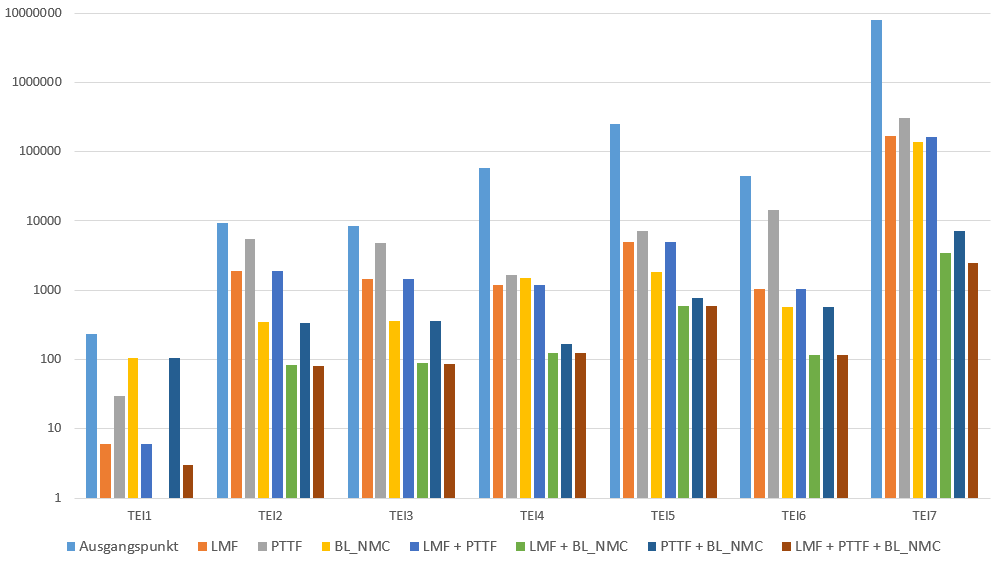
\includegraphics[width=\textwidth]{gegenueberstellung.png}
    \caption{Gegenüberstellung der Untersuchungsergebniss}
    \label{abb:gegenueberstellung}
\end{sidewaysfigure}
